%% 
%% Copyright 2019-2024 Elsevier Ltd
%% 
%% This file is part of the 'CAS Bundle'.
%% --------------------------------------
%% 
%% It may be distributed under the conditions of the LaTeX Project Public
%% License, either version 1.3c of this license or (at your option) any
%% later version.  The latest version of this license is in
%%    http://www.latex-project.org/lppl.txt
%% and version 1.3c or later is part of all distributions of LaTeX
%% version 1999/12/01 or later.
%% 
%% The list of all files belonging to the 'CAS Bundle' is
%% given in the file `manifest.txt'.
%% 
%% Template article for cas-dc documentclass for 
%% double column output.

\documentclass[a4paper,fleqn]{cas-dc}

\usepackage[numbers]{natbib}
\usepackage{subcaption}
\usepackage{tikz}
\usetikzlibrary{calc}

%% --------------------------------
%% | Own Commands                 |
%% --------------------------------
\usepackage{newtxtt}
\newcommand{\Vector}[1]{{\ensuremath{\textbf{\textit{#1}}}}}
\newcommand{\Matrix}[1]{{\ensuremath{\textbf{\texttt{#1}}}}}
\newcommand{\TMatrix}[3]{{^{\mathrm{#1}}\Matrix{#2}_{\mathrm{#3}}}}
\newcommand{\Quat}[1]{{\ensuremath{\textbf{#1}}}}
\newcommand{\DQuat}[1]{{\ensuremath{\hat{\Quat{#1}}}}}
\newcommand{\DVector}[1]{{\ensuremath{\hat{\Vector{#1}}}}}
\newcommand{\trans}{\ensuremath{^\top}}

% Author macros
\def\tsc#1{\csdef{#1}{\textsc{\lowercase{#1}}\xspace}}
\tsc{WGM}
\tsc{QE}

\begin{document}
\let\WriteBookmarks\relax
\def\floatpagepagefraction{1}
\def\textpagefraction{.001}

% Short title
\shorttitle{MocapGS: Robust Online 3D Mapping Using Motion Capture and Gaussian Splatting}    

% Short author
\shortauthors{Theodor Kapler et al.}  

% Main title of the paper
\title [mode = title]{MocapGS: Robust Online 3D Mapping Using Motion Capture and Gaussian Splatting}  

% Authors
\author[1]{Theodor Kapler}%[<options>]
\cormark[1]
\ead{theodor.kapler@student.kit.edu}
\affiliation[1]{organization={Institute of Photogrammetry and Remote Sensing, Karlsruhe Institute of Technology},
            addressline={Englerstr. 7}, 
            city={Karlsruhe},
            postcode={76131}, 
            state={Baden-Württemberg},
            country={Germany}}

\author[1]{Markus Hillemann}[orcid=0000-0002-8906-0450]
\ead{markus.hillemann@kit.edu}

\author[1]{Robert Langendörfer}
\ead{robert.langendoerfer@kit.edu}

\author[1]{Markus Ulrich}[orcid=0000-0001-8457-5554]
\ead{markus.ulrich@kit.edu}

% Corresponding author text
\cortext[1]{Corresponding author}

% Abstract
\begin{abstract}
Image-based online 3D mapping allows scenes to be reconstructed incrementally, with new images continuously integrated to provide direct feedback on the reconstructed scene. However, many online reconstruction methods, typically SLAM-applications, rely on image-based camera pose estimation, which is prone to drift and loop-closure errors. To address this issue, we present MocapGS, an online 3D reconstruction method that directly integrates accurate camera poses obtained from a Motion Capture system directly into a 3D Gaussian Splatting-based reconstruction pipeline. By decoupling pose estimation from scene reconstruction, MocapGS leverages externally provided, metrically accurate camera poses to improve robustness and global consistency. To enable this integration, a complete workflow is developed, including temporal synchronization between the camera and the Motion Capture system, camera calibration, hand-eye calibration, and online reconstruction from sequential image-pose pairs. The proposed method is evaluated on multiple datasets and compared to methods estimating poses from image data. Experimental results show that MocapGS yields more stable camera trajectories and improved reconstruction quality compared to such methods, particularly with respect to global consistency. The results demonstrate that Motion Capture can serve as a reliable primary source of camera poses for online 3D reconstruction, highlighting the potential of Motion Capture-driven reconstruction pipelines.
\end{abstract}

% Keywords
\begin{keywords}
Online 3D Reconstruction \sep Motion Capture \sep Gaussian Splatting \sep Time Synchronization \sep Camera Calibration \sep Hand-eye Calibration
\end{keywords}

\maketitle

% Main text
\section{Introduction}\label{sec:introduction}
Image-based 3D reconstruction has become a fundamental technology in computer vision, photogrammetry, and robotics, with applications ranging from industrial inspection \cite{steger_machine_2018} over autonomous driving \cite{behley_efficient_2018} to digital heritage preservation \cite{gomes_3d_2014}. As cameras are inexpensive, flexible, and widely available, image-based approaches remain particularly attractive compared to active sensing modalities.

Classical 3D reconstruction pipelines are predominantly batch-based. Methods such as Structure from Motion (SfM) \cite{schonberger_structure--motion_2016} estimate camera poses, intrinsic parameters, and sparse geometry jointly from a complete set of images, followed by a densification step using Multi-view Stereo (MVS) \cite{schonberger_pixelwise_2016} or learning-based representations, like 3D Gaussian Splatting (3DGS) \cite{kerbl_3d_2023}. While these approaches can achieve good reconstruction quality, they fundamentally require all images to be available in advance. As a consequence, they are unsuitable for scenarios where image data is acquired sequentially and where immediate feedback is desired.

Incremental reconstruction approaches address these issues. Simultaneous Localization and Mapping (SLAM)-methods \cite{cadena_past_2016}  estimate camera poses and scene structure on-the-fly, enabling online operation and continuous map expansion as new images arrive. More recently, learning-based scene representations such as 3DGS have been adapted to online image acquisition \cite{meuleman_--fly_2025}. These methods make it possible to visualize a scene in real-time while it is being reconstructed, providing immediate feedback and enabling adaptive data acquisition.

Despite these advantages, online approaches typically estimate camera poses sequentially from image data alone. As a result, they are prone to drift and loop-closure errors, which can accumulate over time and lead to globally inconsistent reconstructions.

In parallel, Motion Capture (Mocap) systems offer an alternative means of camera pose estimation. By tracking a rigid body with a mounted camera, Mocap systems can provide camera poses with high accuracy and global consistency, independent of visual scene content. However, in the context of 3D reconstruction, such systems are rarely used as the primary source of camera pose retrieval. Instead, they are typically employed for benchmarking, validation, or ground truth generation, leaving their potential for direct integration into online reconstruction pipelines largely unexplored.

This thesis aims to fill this gap by introducing \emph{MocapGS}, a method that integrates accurate camera poses obtained from a Mocap system directly into an online 3D reconstruction pipeline based on 3DGS. To enable this integration, we propose a complete workflow consisting of:
\begin{enumerate}
\itemsep=0pt
\item Temporal Synchronization,
\item Camera Calibration,
\item Hand-eye Calibration,
\item Online 3D Reconstruction, and
\item 3D Mesh Extraction.
\end{enumerate}  

The main contributions of this work are threefold. First, we present the proposed workflow for integrating Mocap-based pose estimation into an online 3DGS reconstruction pipeline. Second, we evaluate the accuracy of the temporal synchronization and calibration procedures. Third, we assess the reconstruction quality and compare our approach against standard 3DGS as well as an online method that estimates camera poses solely from image data.

We find that by decoupling pose estimation from scene optimization, MocapGS combines the online visualization and incremental processing capabilities of modern 3DGS-based methods with the robustness and global consistency of Mocap-based camera tracking. 

\section{Related Work}\label{sec:related_work}
In this section, we summarize the related work regarding 3D reconstruction methods, as well as camera tracking with Mocap.

\subsection{3D Reconstruction Using Structure from Motion}\label{ssec:related_work:3d_reconstruction_sfm}
Classical 3D reconstruction pipelines are predominantly batch-based and follow a two-stage processing scheme. In a first stage, SfM is applied to a complete set of images to jointly estimate camera poses, intrinsics, and a sparse 3D point cloud via bundle adjustment.

In a second stage, dense reconstruction is performed using the estimated poses. Traditional photogrammetric methods rely on MVS to densify the sparse reconstruction. Neural Radiance Fields (NeRFs) \cite{mildenhall_nerf_2021}, a more recent learning-based approach, replaces explicit point-based reconstruction with a continuous scene representation, enabling high-quality novel view synthesis. 3DGS adopts a more explicit scene representation based on learned 3D Gaussian ellipsoids, enabling very fast rendering.

While highly accurate, these pipelines share a key limitation: SfM is always required as a preprocessing step and depends on the availability of the full image set. Consequently, such methods are non-incremental and do not support real-time reconstruction or interactive scene exploration.

\subsection{Online 3D Reconstruction}\label{ssec:related_work:online_3d_reconstruction}
Online 3D reconstruction methods aim to process image data sequentially as it becomes available, without prior knowledge of the full dataset. These approaches typically combine pose estimation and mapping in a single, incremental pipeline.

Classical point-based methods such as SLAM estimate camera poses on-the-fly while incrementally building a map of the environment. More recent learning-based methods extend this idea to neural or hybrid scene representations. Approaches such as MonoGS \cite{matsuki_gaussian_2024}, WildGS-SLAM \cite{zheng_wildgs-slam_2025}, or On-the-fly NVS \cite{meuleman_--fly_2025} enable incremental reconstruction and real-time rendering while estimating camera poses directly from incoming images.

A major advantage of online methods is the ability to visualize the scene in real time and to actively densify under-reconstructed regions. However, pose estimation is sequential and therefore depends on previously estimated poses. As a result, these methods are susceptible to drift and loop-closure errors, which can lead to globally inconsistent reconstructions.

\subsection{Camera Tracking with Motion Capture}\label{ssec:related_work:camera_tracking}
Mocap systems provide an alternative source of camera pose information. By rigidly mounting a camera to a set of tracked markers, the pose of the camera can be recovered in real-time with high accuracy after hand-eye calibration. Such systems yield globally consistent poses and are not affected by drift or loop-closure failures.

In the literature, Mocap is most commonly used for validation or ground truth generation rather than as the primary source of camera poses for reconstruction \cite{endres_evaluation_2012, sturm_benchmark_2012, shu_mocap2gt_2026}. 

This work is situated at the intersection of online 3D reconstruction and Mocap-based camera tracking. While online 3D reconstruction methods provide real-time feedback and incremental processing, Mocap offers accurate and globally consistent poses. The combination of these complementary properties motivates the approach presented in this work.

\section{Notation}\label{sec:notation}
This work extensively relies on rigid transformations in three-dimensional space. A rigid transformation in $\mathbb{R}^3$ has six degrees of freedom, comprising three rotational and three translational components. Throughout this paper, we refer to such transformations as \emph{poses}.

Following the standard formulation in projective geometry~\cite{hartley_multiple_2004}, poses are represented by homogeneous transformation matrices of the form
\begin{equation}
    \Matrix{E} =
    \begin{pmatrix}
        \Matrix{R} & \Vector{t} \\
        \mathbf{0}\trans & 1
    \end{pmatrix},
    \quad \Matrix{E} \in \mathbb{R}^{4 \times 4},
\end{equation}
where $\Matrix{R} \in \mathbb{R}^{3 \times 3}$ denotes a rotation matrix and $\Vector{t} \in \mathbb{R}^3$ a translation vector. Throughout this paper, bold, capital, monospaced symbols (e.g., $\Matrix{E}$, $\Matrix{T}$) are used to denote homogeneous transformation matrices representing poses.

The mapping from an arbitrary pose parameterization $\Vector{e}$ (e.g. Euler angles) to its associated homogeneous transformation matrix is denoted by $\Matrix{T}(\Vector{e})$.

To describe the relative pose between two coordinate systems, the notation $\TMatrix{A}{T}{B}$ is used. This denotes the pose of coordinate system $\mathrm{B}$ relative to coordinate system $\mathrm{A}$.

\section{Methodology}\label{sec:methodology}
This section provides a comprehensive overview of the methodology employed in this work. It systematically describes the proposed workflow for performing online 3D reconstruction using a synchronized and calibrated camera–Mocap system. Figure~\ref{fig:methodology_overview} illustrates the complete pipeline. Each component of the workflow is explained in detail throughout the subsequent sections.

\begin{figure*}
	\centering
	\includegraphics[width=\textwidth]{figures/methodology_overview.pdf}
    \caption[Overview of the proposed workflow]{Overview of the proposed workflow. The calibration process yields the latency offset $\Delta t$, the intrinsic parameter vector $\Vector{i}$, as well as the hand-eye pose $\TMatrix{C}{T}{T}$. These quantities then, together with the online acquired images and tool poses $\TMatrix{T}{T}{B}$, enable the 3DGS-based online 3D reconstruction.}
	\label{fig:methodology_overview}
\end{figure*}

\subsection{Definition of a Rigid Body}\label{ssec:methodology:rigid_body}
To enable camera pose tracking with a Mocap system, we attach a camera rigidly to a fixed set of Mocap markers, which is depicted in Figure~\ref{fig:rigid_body}. These markers define a rigid body that can be tracked by the Mocap system. To maintain the analogy to robotics, in the following, we refer to the rigid body as \emph{tool}. The pose of this tool coordinate system (TCS) can continously be tracked by the Mocap system. It differs from the pose of the camera coordinate system (CCS), that we are interested in, by an unknown pose $\TMatrix{C}{T}{T}$, which we call \emph{hand-eye pose}.

\begin{figure}[]
    \centering
    \includegraphics[width=\linewidth]{figures/rigid_body.png}
    \caption{Hand-held rigid body connecting the camera to spatially fixed set of Mocap markers.}
    \label{fig:rigid_body}
\end{figure}

\subsection{Temporal Synchronization}\label{ssec:methodology:temporal_sync}
To ensure temporally matching image-pose pairs, it is essential to synchronize the camera and the Mocap system precisely within the employed computer system. In general, such synchronization can be achieved using either hardware-based or software-based triggering mechanisms. To avoid the additional complexity and overhead of dedicated trigger cabling, a software-based synchronization approach is adopted in this work. 

Our goal therefore is to determine the latency difference $\Delta t$ between the camera and the Mocap system that arises on the workstation connected to both systems. To achieve this, we define an event that is temporally well localized and observable by both the camera and the Mocap system. By measuring the arrival times of this event on the workstation, the latency difference $\Delta t$ can be determined.

Common synchronization events for heterogeneous sensor setups include LED flashes or abrupt motions. However, the temporal resolution of such events is fundamentally limited by the camera frame rate, as they can typically only be detected as present or absent within individual image frames. This limits the achievable temporal precision.

To overcome this limitation, we instead exploit the continuous vertical motion of a Mocap marker as a synchronization signal. The marker's position is directly available from the Mocap data and can also be reliably segmented in the camera stream. From both modalities, we extract time series describing the marker's vertical movement: the vertical coordinate from the Mocap system and the row coordinate of the segmented marker center in the image sequence. We then fit a cubic spline to each time series to obtain a smooth, continuous representation of the motion. By determining the local maxima of the interpolated trajectories, we estimate the precise time points at which the marker reaches its maximum height with sub-frame accuracy. These time instants are subsequently used as high-precision synchronization events.

\subsection{Camera Calibration}\label{ssec:methodology:cc}
After temporally synchronizing the two systems, the camera calibration is performed. This involves estimating the camera's intrinsic parameter vector $\Vector{i}$, as well as the extrinsic parameters for each calibration image $\Vector{e}_i$. We perform camera calibration using multiple images of a checkerboard, which defines a world coordinate system (WCS). The extrinsic parameters $\Vector{e}_i$ to be estimated for each image describe the pose of the WCS relative to the CCS, so the corresponding homogenous transform is denoted as $\left(\TMatrix{C}{T}{W}\right)_i=\Matrix{T}\left(\Vector{e}_i\right)$. Our camera calibration procedure is based on OpenCV~\cite{bradski_g_opencv_2000} and internally consists of an initial parameter estimation followed by a nonlinear refinement.

\begin{figure*}
	\centering
	\includegraphics[width=\textwidth]{figures/transformations.pdf}
    \caption[]{Depiction of our MocapGS setup: The capture volume is depicted by the cuboid with the Mocap tracking cameras at the top. Left shows the relevant coordinate systems and right the relevant transformations between them.}
	\label{fig:transformations}
\end{figure*}

\paragraph{Initial Parameter Estimation.}
For estimating initial parameters, the method of Zhang~\cite{zhang_flexible_2000} is used. Zhang models the projection of a 3D point in the WCS onto the 2D Image Coordinate System (ICS) through the pinhole camera. This allows for a linear model formulation using homogenous coordinates. The model parameters, namely the intrinsic parameters of the pinhole camera $\Vector{i} = \left(f_x, f_y, c_x, c_y\right)$ and the extrinsic parameters of each image $\Vector{e}_i$, can then linearly be determined.

\paragraph{Nonlinear Refinemant.}
In the following stage, the linearly estimated parameters are refined via nonlinear optimization. Therefore, the camera model is not constrained to linearity and can thus be extended to incorporate lens distortions. We choose a polynomial camera model using two radial distortion coefficients $K_1$ and $K_2$ and two decentering distortion coefficients $P_1$ and $P_2$. 

Collecting all parameters, we define the vector
\begin{equation}
    \boldsymbol{\theta} = \left(f_x, f_y, c_x, c_y, K_1, K_2, P_1, P_2, \Vector{e}_1, \dots, \Vector{e}_{n_o}\right),
\end{equation}
which contains all unknowns to be optimized. The distortion parameters $K_1, K_2, P_1$, and $P_2$ are typically small, so we assume initial values of zero. We can now define the residual function
\begin{equation}
    \label{eq:repr_error_ics}
    d_{\mathrm{CC}}(\boldsymbol{\theta}) = \sum_{k=1}^{n_o} \sum_{j=1}^{n_m}
        \left\| \Vector{m}_{j,k} - \boldsymbol{\pi}\!\left( \Vector{M}_j, \boldsymbol{\theta} \right) \right\|_2^2 
        \;\longrightarrow\; \mathrm{min},
\end{equation}
where $\Vector{m}_{j,k}$ denotes the observed 2D ICS coordinate of the $j$-th corner in the $k$-th image. $\Vector{M}_j$ denotes the corresponding 3D WCS coordinate, which is projected into the ICS with the projection $\boldsymbol{\pi}$. The function $d_{\mathrm{CC}}(\boldsymbol{\theta})$ is commonly referred to as the reprojection error, which we minimize using the Levenberg-Marquardt method~\cite{marquardt_algorithm_1963}. After optimization, the reprojection error~\eqref{eq:repr_error_ics} typically yields a residual value of $d_{\mathrm{CC}}\approx 0.5\,\mathrm{px}$ with our used setup.

\subsection{Hand-eye Calibration}\label{ssec:methodology:hec}
During the acquisition of the calibration dataset, we not only capture calibration images but also record the corresponding tool pose from the Mocap system for each image, synchronized via $\Delta t$. This allows us to perform a hand-eye calibration.

Hand-eye calibration refers to the determination of the relative pose between a robot's end effector (tool) and a camera that is rigidly mounted to it~\cite{daniilidis_hand-eye_1999}. Establishing this relationship allows observations made in the CCS to be transformed into the TCS and subsequently into the robot base coordinate system (BCS).

In our case, we want to use hand-eye calbration to estimate the relative pose bewtween the CCS and the TCS, which can be tracked with the Mocap system. This hand-eye pose $\TMatrix{C}{T}{T}$ then allows the tool poses to be corrected, retrieving the camera pose which can then be used for the online 3D reconstruction. Figure~\ref{fig:transformations} illustrates the relevant coordinate systems and transformations in this context. As for the camera calibration, our hand-eye calibration procedure is based on OpenCV and consists of an initial parameter estimation followed by a nonlinear refinement.

\paragraph{Initial Parameter Estimation.}
The linear approach for estimating initial parameters is based on solving the fundamental equation
\begin{equation}
    \label{eq:hec_basic}
    \Matrix{A}\Matrix{X} = \Matrix{X}\Matrix{B}
\end{equation}
for the hand-eye pose $\Matrix{X}=\TMatrix{C}{T}{T}$. \Matrix{A} represents the known motion of the tool between two tool poses $\left(\TMatrix{T}{T}{B}\right)_i$ and $\left(\TMatrix{T}{T}{B}\right)_j$, which are obtained from the Mocap system. \Matrix{B} represents the corresponding known motion between two camera poses $\left(\TMatrix{C}{T}{W}\right)_i$ and $\left(\TMatrix{C}{T}{W}\right)_j$, which are obtained by the preceding camera calibration.

Several methods exist to solve Equation~\ref{eq:hec_basic}. We choose the approach proposed by Daniilidis~\cite{daniilidis_hand-eye_1999}, which uses dual quaternions to represent poses.

For the following nonlinear refinement, we also need an initial estimate of the base-world pose $\Matrix{Y}=\TMatrix{W}{T}{B}$. A reasonable initialization for $\Matrix{Y}$ can be derived by a single pair of tool pose and camera pose using
\begin{equation}
    \Matrix{Y} = \left(\TMatrix{C}{T}{W}\right)_i^{-1}\Matrix{X}\left(\TMatrix{T}{T}{B}\right)_i,
\end{equation}
which can be seen in Figure~\ref{fig:transformations}.

\paragraph{Nonlinear Refinement}
As for the camera calibration, we adopt a method that minimizes a reprojection error. In contrast to camera calibration, we transform a checkerboard point over a transformation chain containing the base-world pose, the tool pose, and the hand-eye pose before projecting it into the ICS. This allows optimizing for the hand-eye pose and base-world pose. We define the parameter vectors
\begin{equation}
    \begin{split}
        \Vector{x} &= \left( \alpha_x, \beta_x, \gamma_x, t_{x,x}, t_{y,x}, t_{z,x} \right),\\
        \Vector{y} &= \left( \alpha_y, \beta_y, \gamma_y, t_{x,y}, t_{y,y}, t_{z,y} \right),
    \end{split}
\end{equation}
which represent a minimal parameterization of the hand-eye pose~$\Matrix{X}=\TMatrix{C}{T}{T}$ and the base-world pose~$\Matrix{Y}=\TMatrix{W}{T}{B}$, respectively. These are the parameters to be optimized. The nonlinear refinement is formulated as the minimization of the reprojection error function
\begin{equation}
    \begin{split}
        \label{eq:hec_repr_error_ics}
        d_{\mathrm{HEC}}(\Vector{x}, \Vector{y})
            &= \sum_{k=1}^{n_o} \sum_{j=1}^{n_m}
                \left\|
                    \Vector{m}_{j,k} -
                    \boldsymbol{\pi}\!\left(
                        \Vector{M}_{j,k}, \Vector{i}
                    \right)
                \right\|_2^2
            \;\longrightarrow\; \min, \\
        \Vector{M}_{j,k} &= \Matrix{T}(\Vector{x})\left(\TMatrix{T}{T}{B}\right)_k\Matrix{T}(\Vector{y})^{-1}
                        \Vector{M}_j,
    \end{split}
\end{equation}
where $\Vector{m}_{j,k}$ denotes the observed 2D image coordinate of the $j$-th calibration point in the $k$-th image. $\Vector{M}_j$ is the corresponding homogenous 3D WCS coordinate, which is transformed to the CCS of the $k$-th image through the transformation chain illustrated in Figure~\ref{fig:transformations}, yielding $\Vector{M}_{j,k}$. $\Vector{M}_{j,k}$ is then projected into the image via the projection function~$\boldsymbol{\pi}$ using the intrinsic camera parameters~\Vector{i}. The reprojection error~\eqref{eq:hec_repr_error_ics} is minimized using the Levenberg-Marquardt algorithm~\cite{marquardt_algorithm_1963}, yielding optimal estimates for both the hand-eye pose~\Matrix{X} and the base-world pose~\Matrix{Y}. After optimization, the reprojection error~\eqref{eq:hec_repr_error_ics} typically yields a residual value of $d_{\mathrm{HEC}}\approx 1.5\,\mathrm{px}$ with our used setup.

\subsection{Online 3D Reconstruction}\label{ssec:methodology:online_3d_reconstruction}
At this stage, the following quantities are available from the preceding synchronization and calibration procedure:
\begin{enumerate}
    \item the latency difference $\Delta t$,
    \item the intrinsic parameter vector $\Vector{i}$,
    \item the hand-eye pose $\TMatrix{C}{T}{T}$.
\end{enumerate}
With these quantities, we can now perform the 3DGS-based online 3D reconstruction. During the incremental reconstruction stage, $\Delta t$ enables us to continuously recieve temporally matched pairs of an image and its corresponding tool pose $\TMatrix{T}{T}{B}$. The obtained image is then, using the previously determined intrinsic parameter vector $\Vector{i}$, undistorted and shifted so that the principle point lies in the image center. In the same time, the tool pose $\TMatrix{T}{T}{B}$ can, togehter with the previously determined hand-eye pose $\TMatrix{C}{T}{T}$, be composed to recieve the desired pose of the BCS with respect to the CCS
\begin{equation}
    \label{eq:methodology:camera_pose_chain}
    \TMatrix{C}{T}{B} = \TMatrix{C}{T}{T} \TMatrix{T}{T}{B}.
\end{equation}
The shifted and undistorted image can then, together with its pose $\TMatrix{C}{T}{B}$, be used as an incremental input to the 3DGS-based online 3D reconstruction to perform reconstruction directly in the BCS.

As a baseline for our reconstruction algorithm, we use the method On-the-fly NVS~\cite{meuleman_--fly_2025}. This approach already handles incremental 3DGS, as well as initial camera pose and intrinsic parameter estimation and their refinement in the 3DGS optimization.

Our goal therefore is to streamline this baseline approach by eliminating the initial camera pose and intrinsic parameter estimation and replacing those by our well-known intrinsic parameter vector $\Vector{i}$ and on-the-fly acquired camera pose $\TMatrix{C}{T}{B}$. This enables us to perform online, incremental 3D reconstruction using 3DGS, already in the metric BCS. 

To investigate whether additional pose refinement is beneficial, we implement and evaluate three different variants. We refer to these methods as follows:

\begin{enumerate}
    \item \textbf{MocapGS-Fixed:} The initial camera poses obtained from the Mocap system are used directly and are not further refined.
    \item \textbf{MocapGS-FullOpt:} The initial camera poses are refined jointly with the Gaussian parameters during the 3DGS optimization.
    \item \textbf{MocapGS-RotOpt:} Only the rotational components of the initial camera poses are refined during 3DGS optimization, while the translational components are kept fixed in order to preserve the metric scale of the reconstruction.
\end{enumerate}

\subsection{3D Mesh Extraction}\label{ssec:methodology:mesh_extraction}
After completing the online 3DGS-based 3D reconstruction, we perform an offline surface extraction step to recover the explicit geometry of the observed scene or object. For this purpose, we adopt the efficient mesh extraction pipeline proposed in SuGaR~\cite{guedon_sugar_2024}, which is straightforward to integrate with a previously trained Gaussian representation.

SuGaR extracts surface points by identifying locations of equal density within the scene. Specifically, multiple depth maps are rendered from different viewpoints, and pixels are sampled from each depth map. For every corresponding camera ray, the method determines whether a point with a predefined density value exists along the ray and, if so, computes its 3D position. The collection of these points yields a sparse sampling of the underlying surface. Finally, Poisson surface reconstruction~\cite{kazhdan_poisson_2006} is applied to the extracted surface points to generate a triangular mesh.

\section{Evaluation}\label{sec:experiments}
This section presents a comprehensive evaluation of the proposed MocapGS method. We first describe the comparative setup and introduce the datasets employed in our experiments. Subsequently, we report both quantitative and qualitative results.

\subsection{Comparative Setup}
We compare our approach against 3DGS, as well as against On-the-fly NVS, which forms the basis of our system. The key difference between the methods lies in how camera poses and intrinsic parameters are obtained and optimized.

3DGS estimates all camera poses and intrinsics in advance using COLMAP~\cite{schonberger_pixelwise_2016}. The comparison is therefore not completely fair, since it is not an online method and is significantly slower. Nevertheless, we include it as a baseline because it represents a strong, widely adopted offline approach.

On-the-fly NVS is an online method and estimates intrinsics from a bundle adjustment of the first 8 frames. Initial camera poses for each subsequent frame are then also estimated using bundle adjustment and refined during the following scene optimization.

MocapGS is also an online method and leverages externally provided and calibrated camera parameters. Camera intrinsics are assumed to be known and fixed, while camera poses are obtained from the Mocap system. To study the influence of pose optimization during training, we evaluate the three variants of our approach, MocapGS-Fixed, MocapGS-FullOpt, and MocapGS-RotOpt.

\subsection{Datasets}
We evaluate all methods on three reconstruction datasets we captured using our Mocap setup:
\paragraph{Buddha.}
This dataset consists of 411 RGB images capturing a Buddha statue from multiple concentric viewpoints, each with its corresponding Mocap pose. The object exhibits both coarse geometric structure and fine-grained surface details, making it well suited for quantitative 3D evaluation. A highly accurate 3D ground truth of the statue is available in the form of a dense mesh acquired using a structured-light scanning system, for details refer to \cite{petrovska_geometric_2023, petrovska_vision_2024}.

\paragraph{Robot.} 
This dataset consists of 409 RGB images, each with an associated Mocap pose. It captures a working table setup that includes a robot arm, controller, monitor, computers, and various cables. The scene is captured from multiple concentric viewpoints. This dataset poses a particularly challenging reconstruction scenario due to its complex and heterogeneous geometry, as well as the presence of thin structures and significant clutter. A 3D ground truth of the working table is available in the form of a dense point cloud acquired using a Zoller+Fröhlich Imager 5016 laser scanner.

\paragraph{PhotoLab.} 
This dataset consists of 176 RGB images capturing the room in which the Mocap system is installed. Each image is accompanied by its corresponding Mocap pose. Unlike the previous datasets, the scene is captured in an eccentric, inside-out manner: instead of observing a single object from the outside, the camera traverses the room along a looped trajectory, capturing the surrounding environment. This dataset is particularly challenging, especially for image-based pose estimation methods, as many visual features are only observed from a limited number of viewpoints. A 3D ground truth of the room is not available.

\subsection{General Considerations}
In contrast to COLMAP and On-the-fly NVS, MocapGS is not constrained to a minimum image overlap for pose estimation. Despite this advantage of MocapGS over COLMAP and On-the-fly NVS, all datasets provide sufficient image overlap, enabling COLMAP and On-the-fly NVS to estimate camera poses for each image.

MocapGS uses the Mocap poses as input, while \\COLMAP+3DGS and On-the-fly NVS only use the captured images as input and infer the pose solely from image data. COLMAP+3DGS and On-the-fly NVS therefore operate with an unknown scale factor, while MocapGS is able to operate in metric units due to the calibrated Mocap system.

\begin{table*}[t]
\centering
\caption{Quantitative results on the Buddha, Robot, and PhotoLab datasets.
We report runtime (including pose estimation), PSNR, SSIM, and $\sigma_{\mathrm{3D}}$.
The \colorbox{blue!50}{\strut best} and \colorbox{blue!20}{\strut second best} results are color-coded among the online methods (On-the-fly NVS and MocapGS variants).}
\resizebox{\textwidth}{!}{
\begin{tabular}{l|cccc|cccc|cccc}
\toprule
 & \multicolumn{4}{c|}{\textbf{Buddha}} 
 & \multicolumn{4}{c|}{\textbf{Robot}} 
 & \multicolumn{4}{c}{\textbf{PhotoLab}} \\
\cmidrule(r){2-5} \cmidrule(r){6-9} \cmidrule(r){10-13}
 & Time$\downarrow$ & PSNR$\uparrow$ & SSIM$\uparrow$ & $\sigma_{\mathrm{3D}}$ (mm)$\downarrow$
 & Time$\downarrow$ & PSNR$\uparrow$ & SSIM$\uparrow$ & $\sigma_{\mathrm{3D}}$ (mm)$\downarrow$
 & Time$\downarrow$ & PSNR$\uparrow$ & SSIM$\uparrow$ & $\sigma_{\mathrm{3D}}$ (mm)$\downarrow$ \\
\midrule
On-the-fly NVS
& 02:00 & 29.10 & \cellcolor{blue!20}0.83 & 6.2
& 01:58 & 26.17 & 0.82 & \cellcolor{blue!20}4.5
& 00:45 & 25.89 & \cellcolor{blue!20}0.78 & -- \\

MocapGS-Fixed
& \cellcolor{blue!50}01:53 & 28.80 & 0.82 & \cellcolor{blue!20}5.4
& \cellcolor{blue!50}01:52 & 26.82 & 0.83 & 4.7
& \cellcolor{blue!50}00:42 & 31.52 & \cellcolor{blue!50}0.85 & -- \\

MocapGS-FullOpt
& \cellcolor{blue!20}01:55 & \cellcolor{blue!50}29.56 & \cellcolor{blue!50}0.84 & \cellcolor{blue!50}5.1
& \cellcolor{blue!20}01:53 & \cellcolor{blue!50}28.05 & \cellcolor{blue!50}0.85 & \cellcolor{blue!50}4.2
& \cellcolor{blue!20}00:43 & \cellcolor{blue!50}31.73 & \cellcolor{blue!50}0.85 & -- \\

MocapGS-RotOpt
& \cellcolor{blue!20}01:55 & \cellcolor{blue!20}29.47 & \cellcolor{blue!50}0.84 & \cellcolor{blue!50}5.1
& 01:54 & \cellcolor{blue!20}27.61 & \cellcolor{blue!20}0.84 & 5.0
& \cellcolor{blue!20}00:43 & \cellcolor{blue!20}31.68 & \cellcolor{blue!50}0.85 & -- \\
\midrule
COLMAP + 3DGS
& 12:42 & 31.67 & 0.92 & 14.2
& 12:06 & 31.53 & 0.93 & 7.0
& 11:13 & 32.14 & 0.90 & -- \\
\bottomrule
\end{tabular}
}
\label{tab:reconstruction_results}
\end{table*}

\begin{figure*}
	\centering
	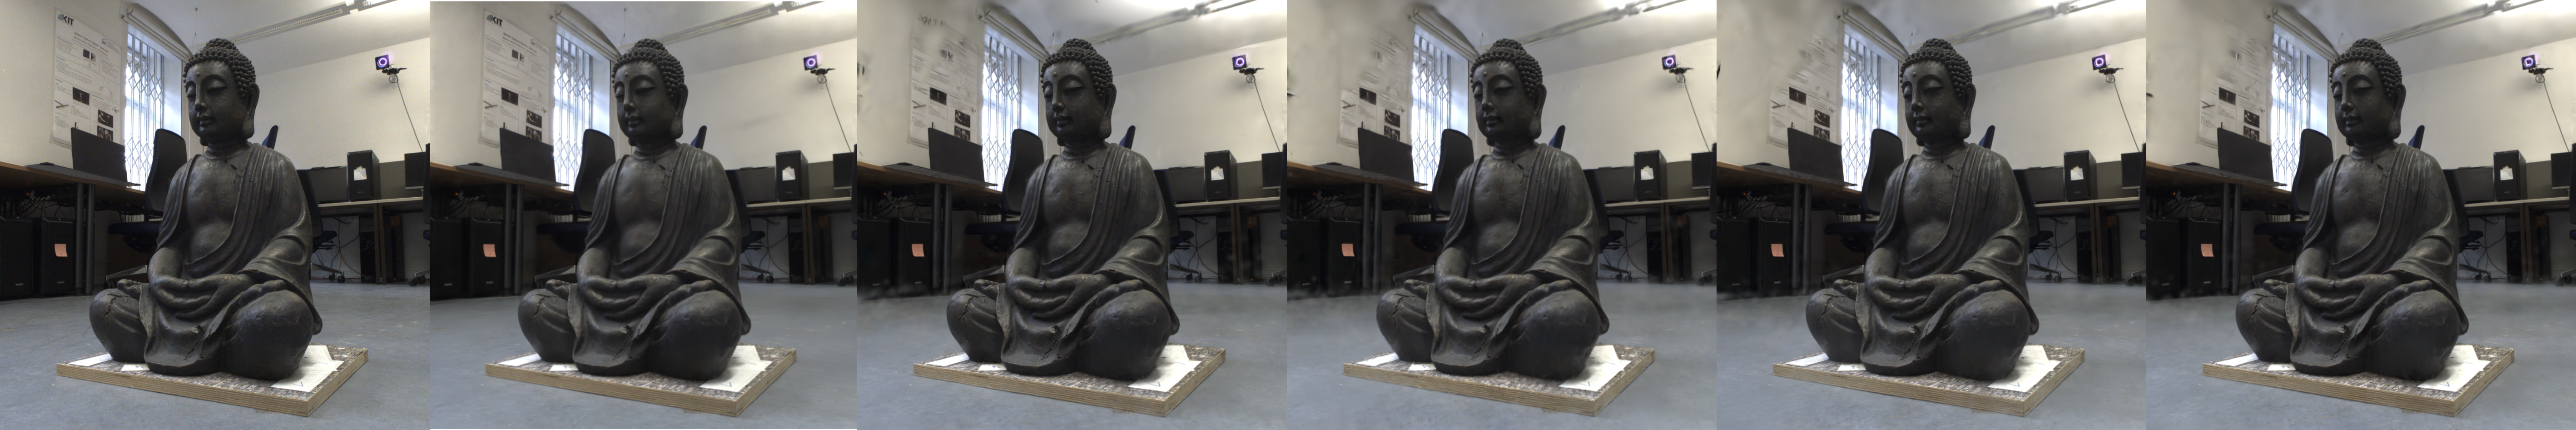
\includegraphics[width=\textwidth]{figures/buddha_montage.png} \\
    \vspace{0.1cm}
    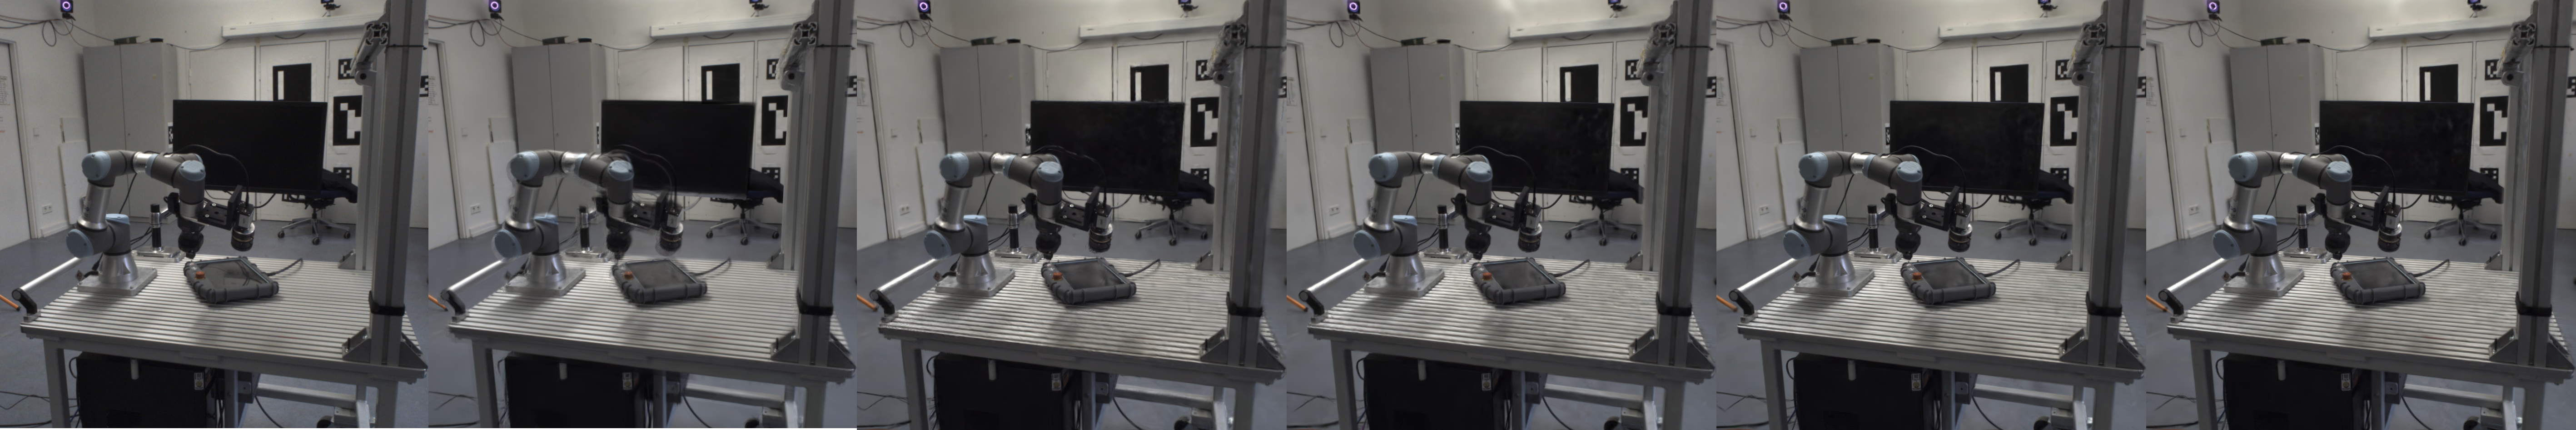
\includegraphics[width=\textwidth]{figures/robot_montage.png} \\
    \vspace{0.1cm}
    \includegraphics[width=\textwidth]{figures/photolab_montage.png}

    \begin{minipage}[t]{0.16\linewidth}
        \centering
        Ground Truth
    \end{minipage}
    \begin{minipage}[t]{0.16\linewidth}
        \centering
        3DGS
    \end{minipage}
    \begin{minipage}[t]{0.16\linewidth}
        \centering
        On-the-fly NVS
    \end{minipage}
    \begin{minipage}[t]{0.16\linewidth}
        \centering
        MocapGS-Fixed
    \end{minipage}
    \begin{minipage}[t]{0.16\linewidth}
        \centering
        MocapGS-FullOpt
    \end{minipage}
    \begin{minipage}[t]{0.16\linewidth}
        \centering
        MocapGS-RotOpt
    \end{minipage}
    \caption{Test image that has not been used during training (left) and rendered scene for all corresponding methods. Buddha dataset on top, Robot dataset in the middle and PhotoLab dataset below.}
	\label{fig:2d_results}
\end{figure*}

\subsection{Metrics}
\paragraph{2D Metrics.}
For assessing the rendering quality of the output 3DGS representation, we report the Peak Signal-to-Noise Ratio
(PSNR) and Structural Similarity Index Measure (SSIM). These metrics are computed using ground truth image-pose pairs, that have not been used for training. 

For COLMAP+3DGS, we use the camera poses estimated from COLMAP as ground truth pose.

On-the-fly NVS jointly optimizes camera poses and the scene representation. Consequently, a strict separation between scene representation and ground truth poses is less straightforward. In their evaluation protocol, the authors estimate the poses of test images during joint 3DGS optimization while keeping the scene representation fixed, resulting in no scene update for a given test image-pose pair.

For MocapGS-Fixed, we use the camera poses acquired by the Mocap system as ground truth pose. MocapGS-FullOpt and MocapGS-RotOpt further refine the test poses similar to On-the-fly NVS.

\paragraph{3D Metrics.}
For the 3D evaluation, we convert the optimized 3DGS representation into an explicit triangle mesh following the procedure described in Section~\ref{ssec:methodology:mesh_extraction}. The reconstructed mesh is then compared to the ground truth 3D data, which consists of a triangle mesh for the Buddha dataset and a point cloud for the Robot dataset.

Before comparison, we align the reconstructed mesh to the ground truth using a two-stage registration procedure: an initial coarse alignment based on manually selected point correspondences, followed by fine registration using the Iterative Closest Point (ICP) algorithm~\cite{besl_method_1992}. We then compute Cloud-to-Mesh (C2M) distances.

For the Buddha dataset, C2M distances are measured from the reconstructed mesh vertices to the ground truth mesh. For the Robot dataset, due to the sparsity of the ground truth point cloud, distances are computed from the ground truth points to the reconstructed mesh.

From all C2M distances, the mean $\mu_{\mathrm{3D}}$ and standard deviation $\sigma_{\mathrm{3D}}$ can be calculated. In principle, $\mu_{\mathrm{3D}}$ should be small if the reconstructed mesh is registered perfectly to the ground truth. $\mu_{\mathrm{3D}}$ therefore serves as a measure of the quality of the registration. The residual uncertainty and noise are characterized by the standard deviation $\sigma_{\mathrm{3D}}$, which therefore is the metric we report.

\subsection{Quantitative Evaluation}

Table~\ref{tab:reconstruction_results} summarizes the numerical reconstruction results for all compared methods. We report all previously introduced evaluation metrics as well as the training duration for each approach. For 3DGS, the reported training duration corresponds to 30,000 optimization iterations. Since 3DGS is not incremental, we additionally account for the preprocessing time required for pose estimation using COLMAP.

For On-the-fly NVS and our MocapGS variants, the training duration is measured as the cumulative runtime after performing 30 iterations per sequential input image. As all datasets are pre-captured and include recorded Mocap poses, these timings represent a best-case runtime scenario for the respective methods.

Considering the 2D evaluation metrics PSNR and SSIM, 3DGS consistently achieves the highest scores across all datasets. This performance, however, comes at the cost of substantially longer training times due to the additional COLMAP overhead and the fixed number of optimization iterations. Among the four online methods, we observe that MocapGS-FullOpt and MocapGS-RotOpt consistently outperform On-the-fly NVS by a noticeable margin. This behaviour is especially distinctive on the PhotoLab dataset, which is particularily challenging for image-based pose estimation.

Turning to the 3D evaluation metric $\sigma_{\mathrm{3D}}$ for the Buddha and Robot datasets, it becomes evident that 3DGS is not competitive with respect to extracted 3D geometry. This is likely due to a mismatch between the scene representation learned by 3DGS and our employed surface extraction strategy. Among the four online methods, the lowest $\sigma_{\mathrm{3D}}$ values, and thus the most accurate and stable 3D reconstructions, are consistently achieved by MocapGS variants, highlighting their advantage for high-quality 3D surface extraction.

\begin{figure*}
	\centering
	\includegraphics[width=\textwidth]{figures/buddha_montage_3d.png} \\
    \vspace{0.1cm}
    \includegraphics[width=\textwidth]{figures/robot_montage_3d.png}

    \begin{minipage}[t]{0.16\linewidth}
        \centering
        Ground Truth
    \end{minipage}
    \begin{minipage}[t]{0.16\linewidth}
        \centering
        3DGS
    \end{minipage}
    \begin{minipage}[t]{0.16\linewidth}
        \centering
        On-the-fly NVS
    \end{minipage}
    \begin{minipage}[t]{0.16\linewidth}
        \centering
        MocapGS-Fixed
    \end{minipage}
    \begin{minipage}[t]{0.16\linewidth}
        \centering
        MocapGS-FullOpt
    \end{minipage}
    \begin{minipage}[t]{0.16\linewidth}
        \centering
        MocapGS-RotOpt
    \end{minipage}

    \vspace{0.5cm}
    
    \begin{tikzpicture}
        \node[anchor=south west, inner sep=0] (cbar) 
            {\includegraphics[width=0.4\linewidth]{figures/cbar.png}};
        \foreach \x in {-3,-2.5,-2,-1.5,-1,-0.5,0,0.5,1,1.5} {
            \pgfmathsetmacro{\pos}{(\x + 3)/4.5} 
            \node[below] at ($(cbar.south west)!\pos!(cbar.south east)$) {\footnotesize \x};
        }
    \end{tikzpicture}
    \caption{Extracted 3D geometry of the Buddha dataset (top) and the Robot dataset (bottom) colored according to the C2M distances to the ground truth representation. Color bar in cm.}
	\label{fig:3d_results}
\end{figure*}

\subsection{Qualitative Evaluation}
Figure~\ref{fig:2d_results} shows one test view for each dataset. The ground truth image is depicted along with the rendered views generated from all compared methods from the repsective ground truth pose of the image. Overall, all methods produce visually compelling novel views, which is also reflected in reasonably high PSNR and SSIM values in Table~\ref{tab:reconstruction_results}. Noticable blur can only be observed on the PhotoLab dataset reconstructed by On-the-fly NVS. 

Figure~\ref{fig:3d_results} shows the generated 3D geometry for the Buddha and the Robot dataset. The 3D representations are colored according to their C2M distances to the ground truth. It becomes evident that 3DGS in combined with our employed mesh extraction strategy does not produce a compelling 3D mesh. All other methods procuce visually compelling meshes with an accuracy in the range of few millimeters.

Figure~\ref{fig:photolab_topview_comparison} presents a top-view comparison of the estimated camera poses for the PhotoLab scene. The MocapGS poses are directly provided by the Mocap system, the 3DGS poses are obtained via COLMAP, and the On-the-fly NVS poses are estimated online. MocapGS and 3DGS show close overall agreement, although 3DGS exhibits several outliers. In contrast, the On-the-fly NVS approach suffers from significant pose drift, resulting in a noticeable loop-closure error.

Figure~\ref{fig:photolab_scene} illustrates the impact of this drift on the reconstructed scene. The figure provides an external view of the 3DGS-based representation of the PhotoLab scene. MocapGS produces a geometrically consistent and coherent reconstruction. While 3DGS encounters difficulties at loop closure, leading to local inconsistencies, the On-the-fly NVS reconstruction is globally distorted due to accumulated pose errors.

\begin{figure*}[]
    \centering
    \includegraphics[width=\linewidth]{figures/photolab_trajectories.png}

    \begin{minipage}[t]{0.20\linewidth}
        \centering
        MocapGS-Fixed
    \end{minipage}%
    \hfill
    \begin{minipage}[t]{0.30\linewidth}
        \centering
        3DGS
    \end{minipage}%
    \hfill
    \begin{minipage}[t]{0.5\linewidth}
        \centering
        On-the-fly NVS
    \end{minipage}

    \caption{Top-view comparison of the camera poses in the PhotoLab scene. MocapGS-Fixed poses are obtained directly with the Mocap system, 3DGS poses are estimated with COLMAP, and On-the-fly NVS poses are estimated online.}
    \label{fig:photolab_topview_comparison}
\end{figure*}

\begin{figure*}[]
    \centering
    \captionsetup[subfigure]{labelformat=empty}
    \begin{subfigure}{0.32\textwidth}
        \raggedright
        \includegraphics[width=0.8\linewidth]{figures/scene_mocapgs.png}
        \caption{MocapGS-Fixed}
    \end{subfigure}\hfill
    \begin{subfigure}{0.32\textwidth}
        \centering
        \includegraphics[width=0.8\linewidth]{figures/scene_3dgs.png}
        \caption{3DGS}
    \end{subfigure}\hfill
    \begin{subfigure}{0.32\textwidth}
        \raggedleft
        \includegraphics[width=0.8\linewidth]{figures/scene_onthefly_nvs.png}
        \caption{On-the-fly NVS}
    \end{subfigure}

    \caption{Overview of the Gaussian representation of the PhotoLab scene obtained by MocapGS-Fixed, 3DGS, and On-the-fly NVS.}
    \label{fig:photolab_scene}
\end{figure*}

\section{Discussion}\label{sec:discussion}
\paragraph{MocapGS Variant Selection.}
Among the MocapGS variants, pose optimization clearly improves performance. Both MocapGS-FullOpt and MocapGS-RotOpt outperform \\ MocapGS-Fixed in 2D and 3D metrics, while FullOpt and RotOpt show negligible differences in 2D and 3D metrics. We prefer RotOpt because it optimizes only the rotation while keeping translations fixed, preserving metric scale.

\paragraph{Capture Style.}
On-the-fly NVS, as an example of purely image-based methods, requires an initial pose estimation via bundle adjustment. This restricts newly captured images to small displacements relative to the previous frame. If the user loses track of initial poses, they must reorient the camera toward previously observed regions to re-establish sufficient feature correspondences. This process leads to frequent interruptions during data acquisition. MocapGS addresses this limitation by eliminating the need for initial pose estimation. Initial poses are directly provided by the Mocap system. This enables fully unconstrained camera motion, allowing the user to focus on one part of the scene in one frame and a completely different region in the next without interruption. As a result, our approach enables a seamless, intuitive, and user-friendly data acquisition process.

\paragraph{Robustness.}
Even when disregarding the facilitated capture setup of MocapGS, which allows for sudden and rapid camera movements, and restricting the comparison to datasets with sufficient overlap for On-the-fly NVS to operate, MocapGS proves to be substantially more robust. As shown in Figures~\ref{fig:photolab_topview_comparison} and~\ref{fig:photolab_scene}, the camera poses estimated by On-the-fly NVS often exhibit significant drift or are entirely incorrect, particularly for challenging trajectories such as those in the PhotoLab dataset. This behavior can be attributed to the absence of loop closure in On-the-fly NVS. In contrast, MocapGS effectively exhibits no drift, as its pose estimates do not depend on previous observations but are instead provided continuously with high accuracy by the Mocap system. This design enables robust and stable scene reconstruction even under challenging and complex camera trajectories.

\paragraph{Limitations.}
MocapGS introduces additional overhead compared to the baseline on-the-fly NVS approach. The required synchronization and calibration procedures take approximately five minutes, representing only a modest time investment. However, the financial cost of the motion capture system is significant in comparison to the baseline setup, which requires only a standard camera.

Also, a limitation of the presented approach lies in the separation between reconstruction and surface extraction. While high-quality meshes can be obtained in a post-processing step, the 3DGS representation itself is not explicitly optimized for surface consistency.

\paragraph{Future Work.}
A promising direction for future work is to incorporate surface-aware constraints or loss terms directly into the MocapGS training process, encouraging Gaussians to align with surface structures during reconstruction. Such constraints could improve the quality of the extracted geometry and reduce the reliance on offline surface extraction.

\section{Conclusion}\label{sec:conclusion}
In this paper, we presented MocapGS, a method for online 3D reconstruction that directly integrates accurate camera poses from a Mocap system into a 3DGS-based pipeline. By leveraging globally consistent and metrically accurate Mocap poses, our approach eliminates the need for image-based pose estimation and avoids the requirement for strong image overlap during capture. In comparison to methods that estimate poses solely from visual data, MocapGS achieves a more globally consistent and robust scene reconstruction, avoiding drift and loop-closure issues. Furthermore, the use of metric Mocap poses enables reconstruction in a fully metric scale without additional alignment steps. We hope that this work demonstrates the potential of Mocap systems not only as validation tools, but as primary pose providers for reliable and efficient 3D reconstruction.

% The Appendices part is started with the command \appendix;
% appendix sections are then done as normal sections
%\appendix

%% Bibliography style file
\bibliographystyle{cas-model2-names}

% Bibliography database
\bibliography{references}

\end{document}

